\section{Results}
\label{sec-results}
%\input graphsize_table

We will analyse search performance as follows: 
First, we look at the effectiveness of our new online and offline symmetry
reduction methods using results published in \cite{harabor10} as a 
comparative baseline.
Next, we compare and contrast the performance of our new algorithm with that
of another similar method recently described in the literature \cite{pochter10}.
Finally, we demonstrate the relative strengths and weaknesses of these two
techniques by scaling all maps in our benchmark sets by a factor of 3 and looking
at the effect this has on performance.


\begin{figure*}[t]
       \begin{center}
                       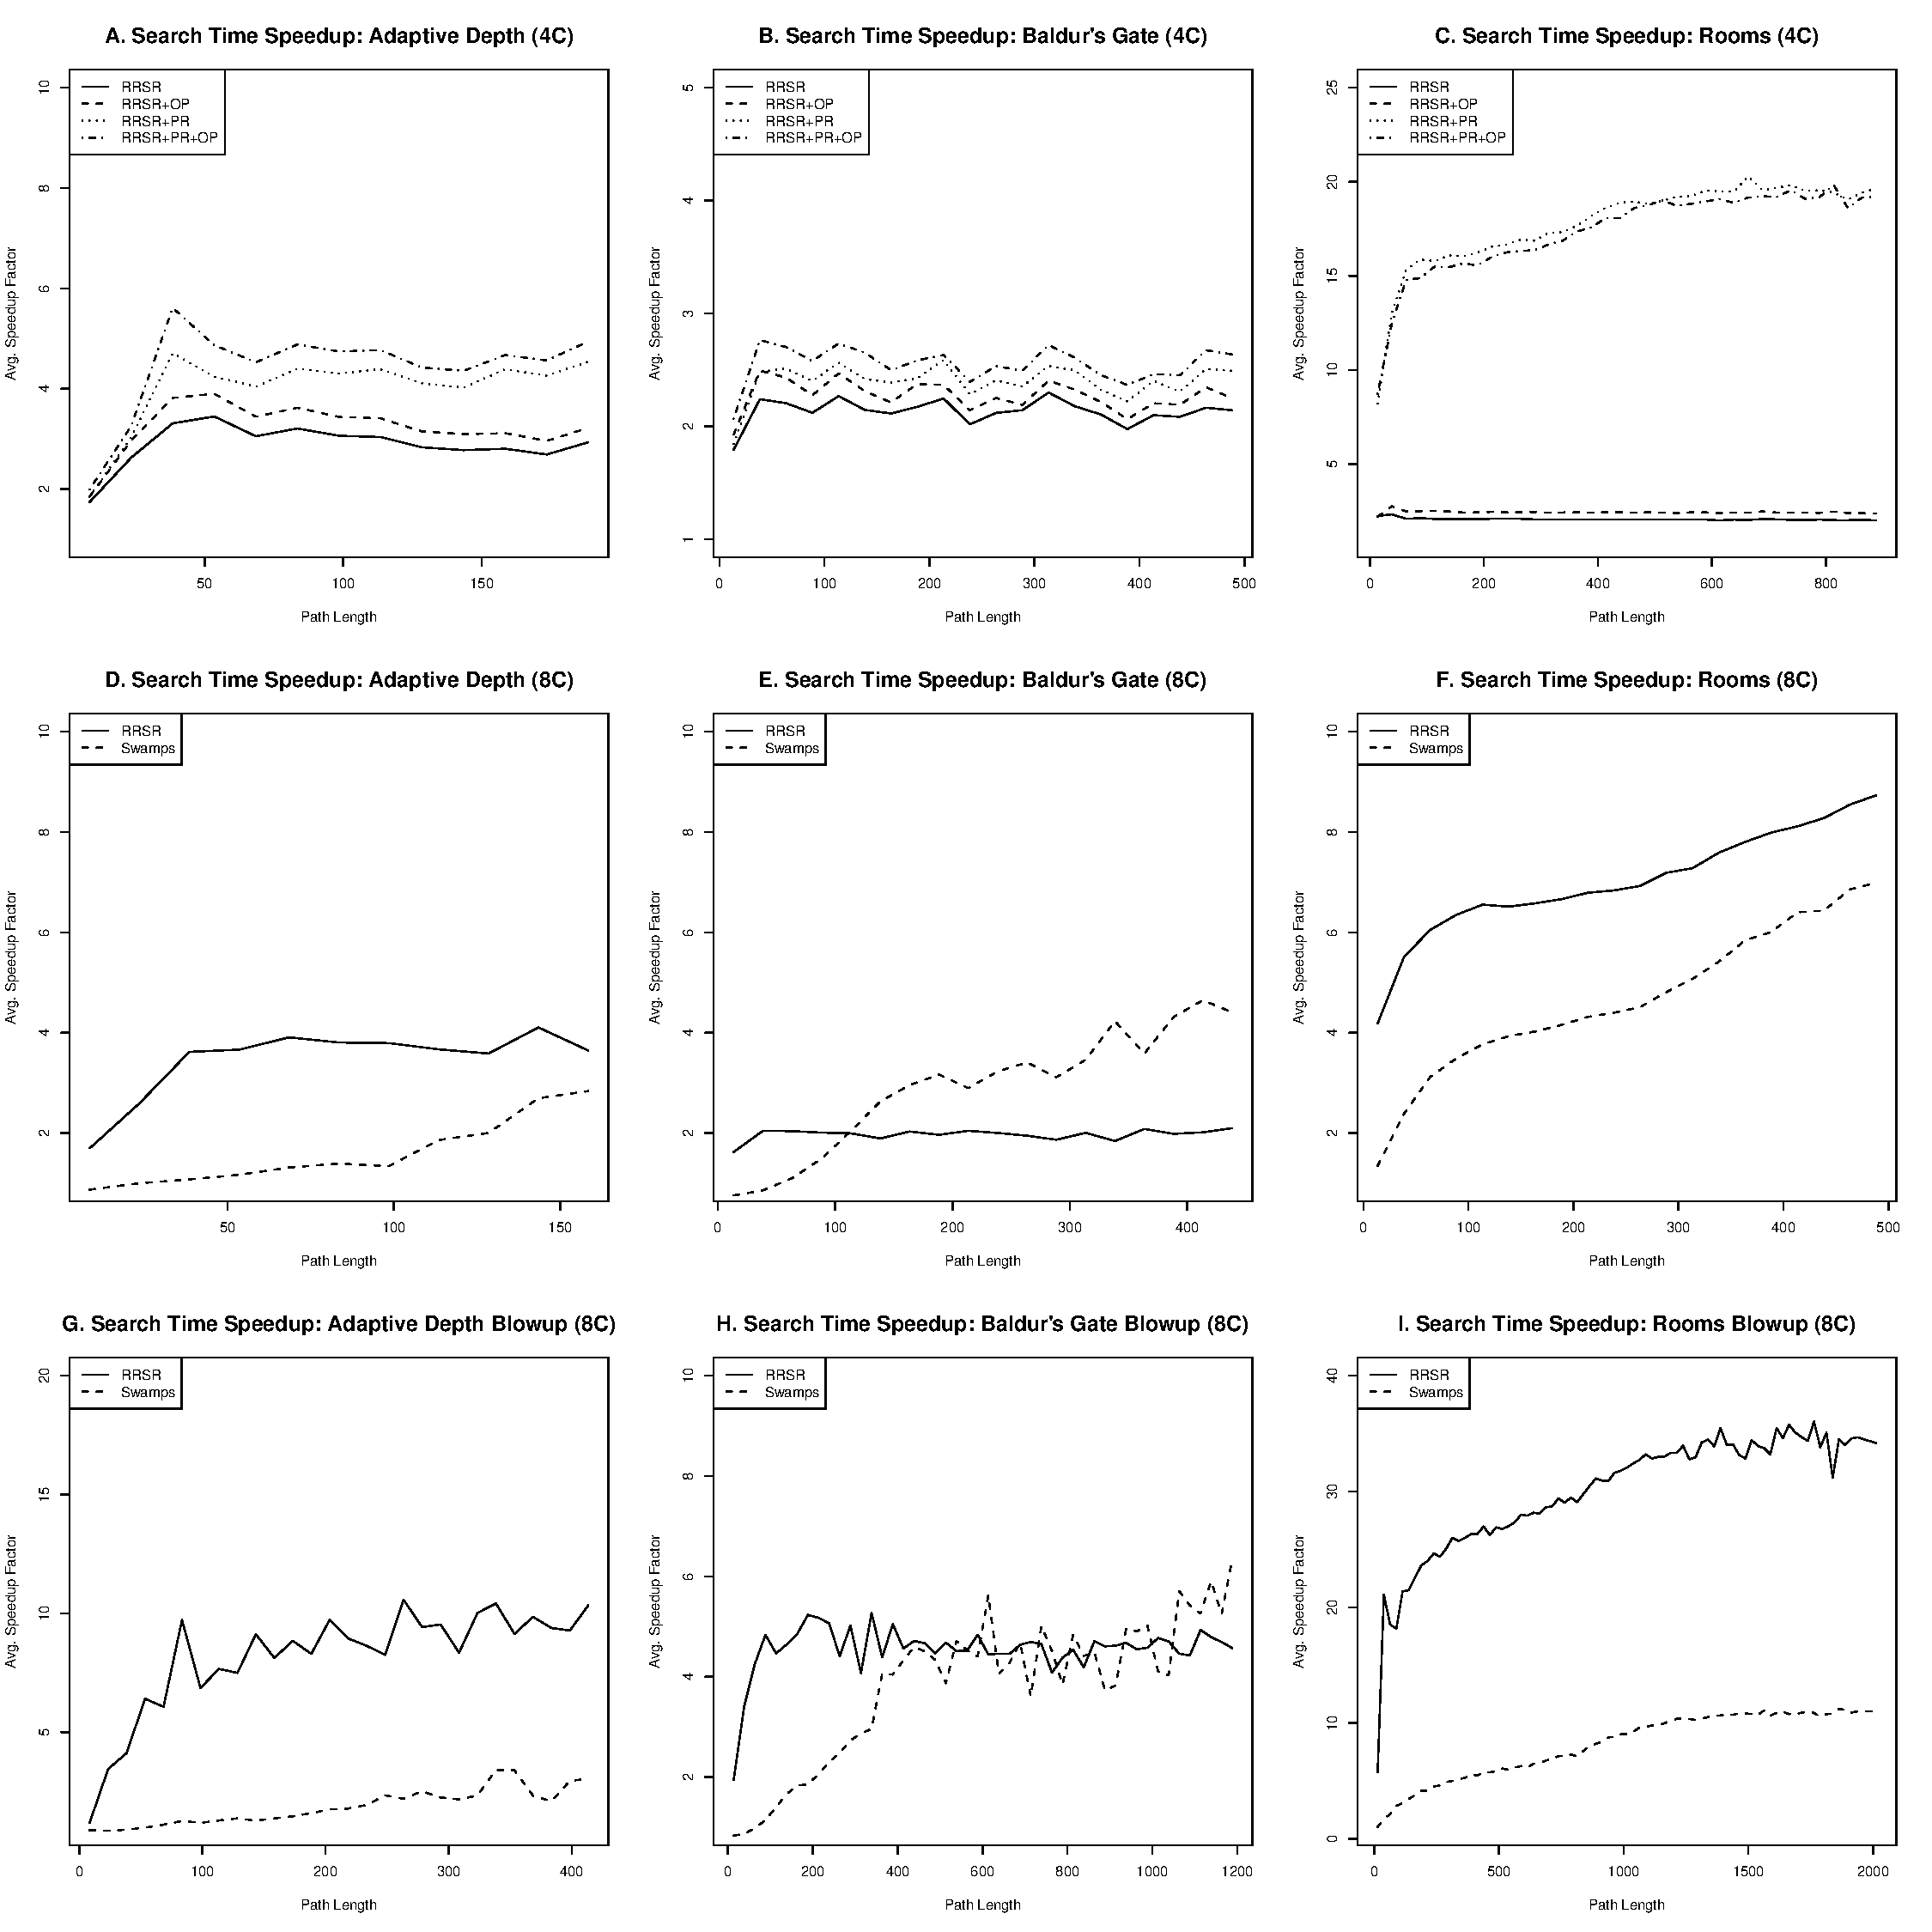
\includegraphics[width=1.95\columnwidth, trim = 10mm 10mm 10mm 0mm]{diagrams/speedup.pdf}
       \end{center}
       \caption{Average A* speedup on each of our three benchmarks. 
		Results are given in terms of search time.}
\label{fig-speedup}
\end{figure*}


\textbf{Comparison with 4ERA and Impact of PR and OP:}
In Figure \ref{fig-speedup} (A to C) we report on the 
effectiveness of offline perimeter reduction (PR) and on-the-fly 
node pruning (OP) to speeding up A*.
Our baseline comparison is the 4ERA algorithm 
originally described by \citeauthor{harabor10}~\shortcite{harabor10}.
Here we restrict our attention to 4-connected grid maps,
since 4ERA does not work on the 8-connected variant.
\par
The charts show a convincing speed-up improvement on all input maps.
In addition, our work broadens the applicability of empty room abstraction
to 8-connected maps.
These two features allow us to conclude that using our enhancements is a better
choice than using 4ERA alone.
\par
It is interesting to note the sometimes large performance variation 
from one benchmark to another. This is indicative of how effectively we can 
decompose the different maps into rectangular shaped regions.
For example, the maps in the Rooms set are highly suited to this approach but those
from Baldur's Gate, which have an unusual 45-degree orientation, are not.
In such cases there are fewer opportunities to build large empty rooms and to apply perimeter reduction.
This leads to larger search spaces and reduced performance. 
\par
When analysing the impact of each enhancement,
we note that the single biggest improvement on each
benchmark is observed when applying perimeter reduction to the basic RRSR method.
In the case of the Rooms benchmark (Figure \ref{fig-speedup}C) RRSR+PR is over 9
times faster than RRSR alone and up to 19 times faster than A* search on an unmodified
grid map.
Smaller but still significant gains are also observed on the remaining two benchmarks:
on Adaptive Depth (Figure \ref{fig-speedup}A) RRSR+PR is twice as fast as RRSR alone
and performance on Baldur's Gate (Figure \ref{fig-speedup}B) is improved by over 10\%.
By comparison, on-the-fly node pruning yields much smaller gains across the same benchmarks.
%both RRSR+OP and RRSR+PR+OP only improve the search performance by 10\% on the majority
%of problem instances.

In an additional experiment, we evaluated the impact of PR and OP on 8-connected grids.
The contribution of OP was much more significant than in the 4-connected case.
This can be explained as follows: on 4-connected maps, 4ERA maintains a very low
branching factor, which is comparable (and even slightly better) than the branching
factor on the original map. On the other hand, 8ERA can introduce larger branching factors.
Therefore, there are more opportunities for on-the-fly pruning in the latter case.
Other details (and charts) are left out because of room limitations.
\par
\textbf{Comparison to Swamps:}
Next, we compare the speedup performance of RSRR+PR+OP with the Swamps algorithm 
described in \cite{pochter10}. Swamps is an alternative search space reduction 
which requires decomposing a graph into so called ``swamp'' areas that can be 
ignored because a there always exists a symmetric path that does not cross any 
tiles in the swamp. 
Each search instance is then limited to an a corridor of inter-dependent 
swamps (and non-swamp areas) and all remaining nodes in the graph are ignored.
To evaluate Swamps we used the authors' source code from \cite{pochter10} and
ran all experiments using their recommended running parameters\footnote{To the best of our knowledge 
these parameters are unpublished; they were recommended to us in a private communique.}:
 a Swamp seed radius of 6 and ``no change limit'' of 2.
\par
Figure \ref{fig-speedup} (D to F) gives search time speedup results for both 
RRSR+PR+OP and Swamps running on the 8-connected variants of our three benchmark 
problem sets. 
On Adaptive Depth (Figure \ref{fig-speedup}D), we observe that 
Swamps yields a maximum search time speedup of 2.8 times faster than 
 A* running on an unmodified grid map; however this is only true for problems of length greater than 150.
By comparison RSRR+PR+OP yields a maximum speedup of 4.1 with comparatively little fluctuation across the
large majority of probem instances.
On Baldur's Gate (Figure \ref{fig-speedup}E) this trend is almost reversed; RRSR+PR+OP consistently 
yields search time speedups of factor 2 while Swamps exhibits a maximum speedup of 4.4.
Finally, on Rooms (Figure \ref{fig-speedup}F) RSRR+PR+OP is again shown to be faster than Swamps;
usually by a factor of between 2 and 3 across most problem instances.
\par
In the benchmarks which RRSR+PR+OP does best (Rooms, Adaptive Depth) 
there are usually large open areas and the terrain can often be naturally decomposed into rectangular rooms.
At the same time, Swamps-based reduction appears to be much better suited for identifying symmetric paths 
in graphs where this is not the case.
\par
\textbf{Effect of Obstacle Density:}
To better understand the effect that obstacle density has on the search performance of the two algorithms
we scaled up each map in every benchmark by a factor of 3.
We then randomly generated a new set of 100 problem instances per map.
%The results are summarized in Figure \ref{fig-speedup} (D to F).
In fhe following analysis we will contrast the new
results with the observed speedup for problems of the same length on the un-scaled maps.
\par
Figure \ref{fig-speedup} (G to I) gives search time speedup performance for both RRSR+PR+OP and Swamps
on each of the scaled-up benchmarks.
On Adaptive Depth (Figure \ref{fig-speedup}G), the average search time speedup of RRSR+PR+OP reaches a maximum of 10. 
By comparison, Swamps reaches a maximum speedup factor of 3.
When we limit our attention to problem instances of length less than 170 we observe that the speedup 
for RRSR+PR+OP has increased, from 4 to 9, when compared to its performance for similar-length problems on the original 
unscaled maps (Figure \ref{fig-speedup}D). 
At the same time, the performance of Swamps has decreased: from 2.8 to 1.2.
Turning our attention to Baldur's Gate (Figure \ref{fig-speedup}H) we observe a similar trend.
Although Swamps has a higher maximum speedup than RRSR+PR+OP (6.4 vs. 5.3), the performance of the two 
algorithms is very similar across a wide range of problem instances (450-1000).
RRSR+PR+OP is clearly faster on instances whose path length is less than 400.
When we limit our attention to problem of length less than 450 we observe that the speedup experienced by
RRSR+PR+OP has increased, from 2 to 4.5, when compared to its performance on the original unscaled maps
(Figure \ref{fig-speedup}E).
Meanwhile, the performance of Swamps has decreased and is now dominated by RRSR+PR+OP.
Finally we turn our attention to the scaled-up Rooms benchmark (Figure \ref{fig-speedup}I).
Here, the increase in size and naturally rectangular topography of the maps in this benchmark
has had a dramatic effect on RRSR+PR+OP speedup, increasing it to over 30 for many instances.
Swamps also exhibits up to a 10 times speedup but if we limit our attention to problems of
length less than 500 we again see a reduction in performance when compared to Swamps speedup
on the original unscaled maps (Figure \ref{fig-speedup}F). 
\par
The observed performance characteristics of both Swamps and RRSR+PR+OP
are not unexpected.
The complementary tendencies of the two algorithms
are consistent with the fact that 
the basic ideas behind swamps and empty room abstraction are quite different.
By definition, a swamp requires that any two nodes adjacent to the swamp
can be connected through an optimal path that does not intersect with the swamp.
In contrast, in the case of empty rectangular rooms, 
crossing the room is the only way to connect optimally nodes on (distinct edges of) the perimeter.
Swamps prune out areas that can be avoided without introducing a detour.
Rectangle abstraction allows for a faster exploration of areas that need to be searched.

In the case of RRSR+PR+OP we would expect performance on an arbitrary grid map to improve as bigger
rooms can be identified and constructed. 
Larger rooms allow us to prune a larger number of interior tiles and we would expect this to be reflected
by an associated increase in speedup. This was indeed the case in our measurements.
In the case of Swamps, we would expect the opposite to occur. As the average size of each swamp increases
there are more tiles to be considered per search. Since the algorithm does not attempt to speed up searching
\emph{inside} a swamp, each swamp traversal takes longer and we would expect to see this reflected
by an associated decrease in speedup. As before, this was indeed the case.

It therefore appears that the two algorithms are orthogonal.
A natural extension of this work would thus be to create a new symmetry-based search space reduction
which combines the two: first, apply RRSR+PR to a grid in order to eliminate as many interior tiles 
as possible; then, apply a Swamps-based decomposition to the resultant graph.

